\documentclass[conference]{IEEEtran}
\IEEEoverridecommandlockouts
% The preceding line is only needed to identify funding in the first footnote. If that is unneeded, please comment it out.
\usepackage{cite}
\usepackage{amsmath,amssymb,amsfonts}
\usepackage{algorithmic}
\usepackage{graphicx}
\usepackage{textcomp}
\usepackage{xcolor}
\def\BibTeX{{\rm B\kern-.05em{\sc i\kern-.025em b}\kern-.08em
    T\kern-.1667em\lower.7ex\hbox{E}\kern-.125emX}}
\begin{document}

\title{ADLR WS21 - Final Report Team 04 \\ Harnessing Reinforcement Learning for Neural Motion Planning\\
}

\author{\IEEEauthorblockN{Marc Hauck}
\IEEEauthorblockA{\textit{Robotics, Cognition, Intelligence} \\
\textit{Technical University of Munich}\\
Munich, Germany \\
ge65qoy@mytum.de}
\and
\IEEEauthorblockN{Baris Tura}
\IEEEauthorblockA{\textit{Robotics, Cognition, Intelligence} \\
\textit{Technical University of Munich}\\
Munich, Germany \\
baris.tura@tum.de}}

\maketitle

\section{Experiments}

\subsection{Discrete Environments}

To get familiar with the Stable-Baselines 3 (SB3) library and the environment inherited from the Open AI gym class, we started with an empty 10 x 10 grid world environment with no obstacles. The agent always started in the top left corner and had to find the goal in the bottom right corner by taking one of the actions UP, DOWN, RIGHT, and LEFT. Similar to the approach in \cite{b1}, the reward was set to 1 at the goal and 0 else. Using a discrete observation and action space, the experiments needed only little computation time and the agent was able to overfit to this environment quickly. For all experiments so far, we used the reinforcement learning algorithm Proximal Policy Optimization (PPO), as was suggested by the SB3 documentation.

In a second step, we added obstacles to the environment and initially rewarded a collision with -1. Adding the obstacles led to a massive increase in computation time as they increased the dimension of the observation space depending on the number of obstacles. Additionally, it required changes of the reward function: If the negative reward of a collision was too small compared to the reward for reaching the goal, the agent would ignore the obstacle and step over it. This was still possible because at that point, we did not reset the environment upon collision yet. If the negative reward for colliding was too high compared to the goal reward, the agent would not move at all and stay in its corner. After increasing the number of training steps and finding a good ratio between positive and negative rewards by using binary search, we were able to successfully train the agent in this environment.

\begin{figure}[htbp]
\centerline{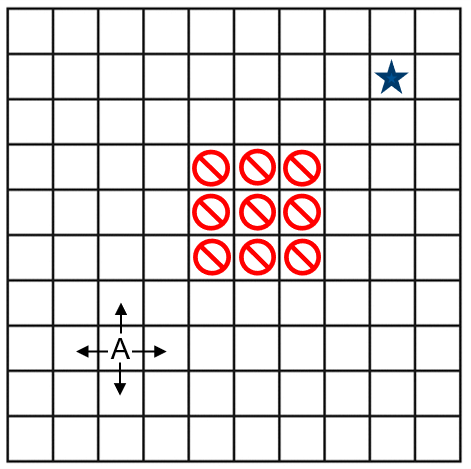
\includegraphics{discrete.png}}
\caption{10x10 discrete environment: The agent (A) has to find the goal (star) without colliding with the obstacles (do-not-cross signs).}
\label{fig1}
\end{figure}

\subsection{Continuous Environments}

Next, we transformed the environment to a continuous one in [0, 10] x [0, 10]. To enable the agent to freely move in the continuous space, the two-dimensional action space was initially set to [-1, 1] for the agent's velocity in x- and y-direction. The experiments started with the sparse rewards from the discrete environment and no obstacles, but the agent was not able to find the goal reliably. As long as the positions of start and goal were fixed, the agent was able to overfit to the goal's position and find it, but if we sampled start and goal position only from small intervals, the agent often went past the goal and ended up stuck in a corner. To overcome this problem, we had to change the reward function in a way that guided the agent more towards the goal. To do that, we rewarded the negative distance of the agent to the goal in every step. This led to good results with little training time.

As in the discrete environment, we then added obstacles and provided a negative reward for a collision. If the agent did not collide, the reward stayed the same as before. We were able to successfully guide the agent to the goal for up to three obstacles, observing an increase of required training time with an increasing number of obstacles again. For environments with more obstacles, the agent was not able to find the goal reliably anymore, even with the training time being one order of magnitude higher than before.

This is caused by the varying size and permutation of the observation space: With each additional obstacle, the dimension of the observation space increases by two, adding another x- and y-position. Furthermore, the permutation of the observation space prevents the agent from gaining a solid understanding of its environment. Even if an obstacle is sampled in the same spot as another obstacle in the run before, the agent may not be able to transfer its knowledge from the previous run to the next due to a possible permutation.

\subsection{Basis Point Sets: An Alternative Obstacle Representation}

To cope with the problems mentioned before, we had to introduce an alternative obstacle representation. We adopted the framework presented in \cite{b2}, where 3D point clouds were projected onto a Basis Point Set (BPS). This BPS consists of a fixed set of so-called basis points that are sampled throughout the environment. Projection of all points onto the BPS yields a distance vector, each entry of the vector representing the distance of the corresponding basis point to the closest point in the cloud, or the closest obstacle respectively. This approach eliminates the issue of varying input shapes as the BPS is predetermined and the resulting vector is always of the same length. It also helps alleviate the problem of possible permutations as each basis point has a fixed corresponding entry in the distance vector.
 
Our best results using this framework were obtained with ten obstacles, the positions of which were projected onto 100 randomly sampled basis points. The agent was able to find the goal in up to 85 out of 100 evaluation runs after the training, albeit colliding at least once in 15 of the cases, which indicates a potential for improvement, although this has been our most successful experiment so far.

\subsection{Environment Representation}

There are three possibilities for representing the environment and specifically the obstacles. The first one is the purely positional one, where for each obstacle the corresponding $x$ and $y$ coordinates are embedded, which leads to a matrix of size $n_{obstacles} \times 2$ as the observation space. This approach is simple and quite easy to compute. Nonetheless, it is also very limited as it lacks expressiveness and does not allow to alter with the number of obstacles in runtime. 
The second option is making use of raw images. Here, at each timestep the environment is rendered, and the resulting RGB tensor is employed as the observation space of the network. This approach is highly expressive. Everything that the agent may need is readily available to it and the agent can have immediate feedback concerning its actions. However, this method leads to a large state space and an accordingly large network. To put in perspective, a square RGB image of size 400 pixels put into use in a DDPG algorithm with 1 million buffer size and 128 batch size requires 437 GB of memory. Making updates to such a big network is cumbersome. 

\begin{figure}[!t]
\centering
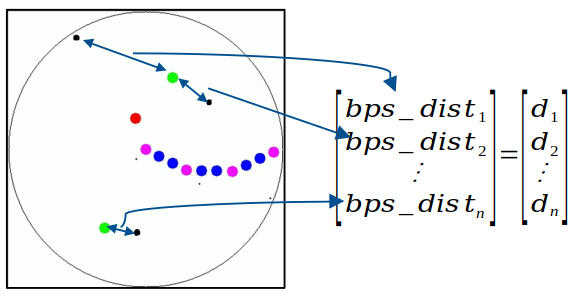
\includegraphics[width=2.5in]{bpsill}
\caption{Basis Points Set as Environment Representation.}
\label{bps_ill}
\end{figure}

The last option is Basis Points Sets, as illustrated in Figure \ref{bps_ill}. This option finds a balance between the other two in terms of expressiveness and simplicity. It is still a relatively expressive method, though not as much as raw images; and it is considerably simple and small in size even though more complex compared to the purely positional representation.

\subsection{Runtime Options}

\begin{figure}[!t]
\centering
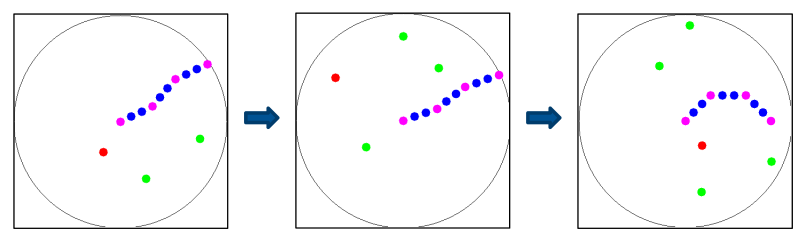
\includegraphics[width=3.2in]{currlearning}
\caption{Curriculum learning concerning number of obstacles. The number of obstacles is increased at each step.}
\label{curr_learn}
\end{figure}

The next set of options concern the runtime and the way learning is done. The first option is the vanilla learning, during which the environment is directly presented to the agent at once, the way it is desired to be in the end. In contrast to that, the other option is curriculum learning, where the learning is kicked off with a relaxed and simple version of the task, and the difficulty is increased as learning progresses. The idea behind curriculum learning is that the agent can carry over what it has learned at each curricular timestep to the next one. Figure \ref{curr_learn} illustrates the concept of curriculum learning applied on number of obstacles in the environment. Here, the environment starts with two obstacles. Once the agent can perform well on two obstacles, it is increased to 3 and consequentially to 4. After the individual transitions between curricular steps, the agent does not need to learn the inverse kinematics again, but only needs to readjust itself according to the changes made in the environment.

\section{Results}

\subsection{Mobile Robot}

\subsection{2 DoF Planar Robot Arm}


\begin{table}[!t]
\renewcommand{\arraystretch}{1.3}
\caption{Results for 2 DoF Planar Robot}
\label{table:1}
\centering
\begin{tabular}{c|ccc|ccc|}
\cline{2-7}
                                  & \multicolumn{3}{c|}{Vanilla}                                       & \multicolumn{3}{c|}{Curriculum}                                    \\ \cline{2-7} 
                                  & \multicolumn{1}{c|}{Positional} & \multicolumn{1}{c|}{BPS} & Image & \multicolumn{1}{c|}{Positional} & \multicolumn{1}{c|}{BPS} & Image \\ \hline
\multicolumn{1}{|c|}{1 Obstacle}  & \multicolumn{1}{c|}{\textbf{84}}          & \multicolumn{1}{c|}{79}   & 70     & \multicolumn{1}{c|}{\textbf{84}}          & \multicolumn{1}{c|}{83}   & 68     \\ \hline
\multicolumn{1}{|c|}{2 Obstacles} & \multicolumn{1}{c|}{64}          & \multicolumn{1}{c|}{68}   & 51     & \multicolumn{1}{c|}{67}          & \multicolumn{1}{c|}{\textbf{70}}   & 54     \\ \hline
\multicolumn{1}{|c|}{3 Obstacles} & \multicolumn{1}{c|}{27}          & \multicolumn{1}{c|}{28}   & 12     & \multicolumn{1}{c|}{27}          & \multicolumn{1}{c|}{\textbf{29}}   & 13     \\ \hline
\end{tabular}
\end{table}



We represent in Table \ref{table:1} the success rate in percentages over a 1000 validation runs for the 2 DoF planar robot. Here, a run is called successful if the agent finds the goal without colliding with any obstacles. The algorithm that was used for these experiments is Proximal Policy Optimization (PPO). We have experimented with Deep Deterministic Gradient Policy (DDPG) and Soft Actor Critic (SAC) as well, yet although these two algorithms show good results very quickly, PPO leads to better results in the long run. As mentioned earlier, the difficult part of this problem is not the complexity of the environment but rather learning the inverse kinematics. As such, we draw attention to comparison cases where the environment elements are kept fixed, that is, different combinations of options for a given number of obstacles. 
For the first case with one obstacle, it is seen that curriculum learning outperforms vanilla learning, with positional representation having a slight edge over BPS, which is to be expected as the usage of more complex BPS representation does not bring about any additional performance for such a simple setting. However, it can also be seen that even for this simple setting the image representation struggles, which gives a hint as to how detrimental large networks can be. 
For the second and third case with two and seven obstacles respectively, we see that the combination of curriculum learning and BPS outperforms all other combinations, with 70\% and 29\%. Based on the above given reasonings, such a result was expected. Even though this is a small set of experiments, we can claim that for the 2 DoF case, the combination of curriculum learning and BPS is the choice to be made. 


\subsection{3 DoF Planar Robot Arm}

\begin{table}[!t]
\renewcommand{\arraystretch}{1.3}
\caption{Results for 3 DoF Planar Robot}
\label{table:2}
\centering
\begin{tabular}{c|ccc|ccc|}
\cline{2-7}
                                  & \multicolumn{3}{c|}{Vanilla}                                       & \multicolumn{3}{c|}{Curriculum}                                    \\ \cline{2-7} 
                                  & \multicolumn{1}{c|}{Positional} & \multicolumn{1}{c|}{BPS} & Image & \multicolumn{1}{c|}{Positional} & \multicolumn{1}{c|}{BPS} & Image \\ \hline
\multicolumn{1}{|c|}{1 Obstacle}  & \multicolumn{1}{c|}{42}          & \multicolumn{1}{c|}{47}   & 39     & \multicolumn{1}{c|}{44}          & \multicolumn{1}{c|}{\textbf{48}}   & 36     \\ \hline
\multicolumn{1}{|c|}{2 Obstacles} & \multicolumn{1}{c|}{30}          & \multicolumn{1}{c|}{35}   & 35     & \multicolumn{1}{c|}{32}          & \multicolumn{1}{c|}{32}   & \textbf{51}     \\ \hline
\multicolumn{1}{|c|}{3 Obstacles} & \multicolumn{1}{c|}{7}          & \multicolumn{1}{c|}{\textbf{13}}   & 10     & \multicolumn{1}{c|}{10}          & \multicolumn{1}{c|}{9}   & 11     \\ \hline
\end{tabular}
\end{table}

Table \ref{table:2} shows the success rate in percentages over a 1000 validation runs for the 3 DoF planar robot. The setting of the algorithms is the same with that of the 2 DoF case. 
Looking at the results, a lack of trend is immediately clear. It should be kept in mind that 3 DoF is much more complicated in comparison to 2 DoF. For the inverse kinematics problem in the 2 DoF setting, there exist two possible solutions for a given point. In contrast to that in the 3 DoF setting, there exist infinitely many solutions, and the agent needs to learn to discern between these many solutions. 
For the one obstacle case BPS and curriculum learning perform the best. Once the number of obstacles is increased to two, suddenly image representation works better and what’s more surprising, for 7 obstacles vanilla learning outperforms curriculum learning. What is happening here is that the agent cannot learn what’s at the core of the task, that is, the inverse kinematics. When such is the case, it does not help any further to employ advanced techniques such as curriculum learning or basis points sets. Thus, we can conclude that for neural motion planning, the inverse kinematics should be learned first, and everything else should follow that. 









\begin{figure}[htbp]
\centerline{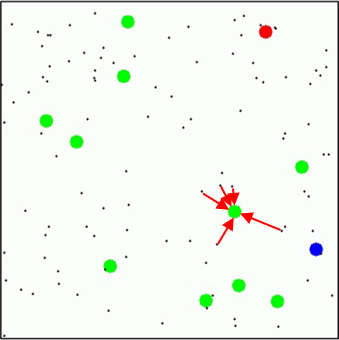
\includegraphics{bps.png}}
\caption{Continuous environment with basis points: The agent (blue) has to find the goal (red) without colliding with the obstacles (green). The red arrows depict the distance to the nearest obstacle of five exemplary basis points (black).}
\label{fig1}
\end{figure}

\section{Conclusion} 

We have shown that for the neural motion planning of a planar robot arm, the main difficulty is not the complexity of the environment but rather learning the inverse kinematics. Through our experiments we have come to the following conclusions
 \begin{itemize}
\item DDPG and SAC show good results very quickly, but PPO proves to be better in the long run.
\item Basis Points Sets provide a good and balanced solution for environment representation
\item Curriculum learning highly enhances the results, as long as the fundamentals can be learned
\end{itemize}
We believe the main and immediate focus of future work should be on learning the inverse kinematics, which can be accomplished by means of supplementing measures such as Hindsight Experience Replay (HER) or expert knowledge in the form of classical path planning. Once that is accomplished, one can move forward and increase the complexity of the environment by increasing the degrees of freedom, making the obstacles dynamic, or transitioning into a 3D environment.


\begin{thebibliography}{00}
\bibitem{b1} T. Jurgenson and A. Tamar, ``Harnessing reinforcement learning for neural
motion planning'',  \textit{arXiv preprint arXiv:1906.00214}, 2019.
\bibitem{b2} S. Prokudin, C. Lassner, and J. Romero. "Efficient learning on point clouds with Basis Point sets". \textit{Proceedings of the IEEE/CVF International Conference on Computer Vision (ICCV)}, pp. 4332–4341, 2019.
\end{thebibliography}

\end{document}

